\chapter{Evaluation}
\label{sec:Evaluation}

%\remark{
%{\em Expected Outcome:} Reader believes that participatory networking provides 
%benefits to real applications, and that it is feasible to implement such a 
%system in today's networks.
%}

We evaluate our \sys prototype with the Mininet platform for
emulating SDNs~\cite{Mininet}, and with real networks. Our primary
testbed includes two Pronto 3290 switches %running the Indigo
%firmware,\footnote{\scriptsize{\url{http://indigo.openflowhub.org/}}}
and several software OpenFlow switches (both Open vSwitch and the
reference user-mode switch) %running
on Linux Intel-compatible
hardware, and on the TP-Link WR-1043ND wireless router.  Wired
connections are 1 Gbps and wireless runs over 802.11n. Clients on
the network include dedicated Linux servers, and fluctuating numbers
of personal laptops and phones. In addition to the participatory
networking API, the network also provides standard services such as
DHCP, DNS, and NAT.

Members of our group have been using the testbed since February 2012
to manage our traffic, and during this time, it has
been our primary source of network connectivity. The testbed is
compatible with unmodified consumer electronic devices, which can
easily interact with a \sys controller running at a well-known
location.\footnote{The \sys controller could also be specified using
a DHCP vendor-specific or site-specific option.}

In the following chapters, we examine two aspects of our prototype.
First, we consider four case studies of real applications
that use the \sys API to improve end-user experience
(\xref{sec:ApplicationUsage}).  Second, we evaluate the practicality
of implementing the \sys API in current OpenFlow-enabled networks,
considering questions such as the latency of processing requests,
and the number of rules created by networked applications
(\xref{sec:Microbenchmarks}).

\section{Application Usage}
\label{sec:ApplicationUsage}

We ported four real applications to use the \sys API: Ekiga,
SSHGuard, ZooKeeper, and Hadoop. We now describe how intentions of
an application developer or user can be translated to our API, and
the effects of using \sys on the network and the application. Our
\sys-enabled versions of these applications are all publicly
available on Github.\footnote{\url{http://github.com/brownsys}.}

\subsection{Ekiga}

Ekiga is an open source video conferencing application. %\footnote{http://ekiga.org}
We modified Ekiga to ask the user for the anticipated duration of
video calls,
% when it is placed.
and use a \priv{Reserve} message to request guaranteed bandwidth
from the network between the caller's host and either the network
gateway or the recipient's host, for the appropriate time. If such a
reservation is not available, Ekiga retrieves the schedule of
available bandwidth from \sys and calculates the earliest time at
which a video call or, alternatively, an audio call, can be made
with guaranteed quality. It then presents these options to the
user, along with a third option for placing a ``best effort'' call
right away.
%Our modified version of Ekiga is available on Github.

Realizable reservations cause the \sys controller to create
guaranteed bandwidth queues along the path of the circuit, and
install forwarding rules for Ekiga's traffic.

Measurements of Skype use on a campus network with more than 7000
hosts show that making reservations with \sys for VoIP applications
is quite feasible. Skype calls peaked at 75 per hour, with 80\% of
calls lasting for fewer than 30 minutes~\cite{SkypeTraffic}.  This
frequency is well within current OpenFlow switches' capabilities, as
we measure in \xref{sec:Microbenchmarks}.\\

\subsection{SSHGuard}
\label{sec:sshguard}

SSHGuard is a popular tool to detect brute-force attacks via log monitoring
and install local firewall rules (\eg, via \verb/iptables/)
in response. We modified SSHGuard to use
\sys as a firewall backend to block nefarious traffic entering
the network. In particular, this means such traffic no longer traverses the
targeted host's access link.

For example, if Alice is running SSHGuard on her host and
it detects a Linux syslog entry such as:

\begin{small}
\begin{verbatim}
sshd[2197]: Invalid user Eve from 10.0.0.3
\end{verbatim}
\end{small}
%
SSHGuard will block Eve's traffic for the next five minutes using
\sys's \priv{Deny} request. The \sys controller then places an
OpenFlow rule to drop packets to Alice's host coming from Eve's at a
switch close to Eve's host.
%, following the procedure in \xref{sec:NIB}.

Although this is a basic example, it illustrates \sys's ability to
expose in-network functionality (namely, dropping packets) to
end-user applications.  Besides off-loading work from the end-host's
network stack, this approach also protects any innocent traffic
which might have suffered due to sharing a network link with a
denial-of-service (DoS) attack.

To demonstrate this benefit, we generated a UDP-based DoS attack
within our testbed network. We started an \verb/iperf/ TCP transfer between
two wireless clients, measured initially at 24 Mbps. We then
launched the attack from a Linux server two switch-hops away from
the wireless clients. During the attack, which was directed at one
of the clients, the performance of the \verb/iperf/ transfer dropped to 5
Mbps, rising to only 8 Mbps after the victim installed a local
firewall rule.  By using \sys to block the attack, the transfer's
full bandwidth returned.

\subsection{ZooKeeper}

ZooKeeper~\cite{Hunt:2010} is a coordination service for distributed systems 
used by Twitter, Netflix, and Yahoo!, among others, and is a key component of 
HBase. Like other coordination services such as Paxos~\cite{Lamport:1998}, 
ZooKeeper provides consistent, available, and shared state using a quorum of 
replicated servers (the \emph{ensemble}). For resiliency in the face of network 
failures, ZooKeeper servers may be distributed throughout a datacenter, and 
thus quorum messages may be negatively affected by heavy traffic on shared 
links. Because ZooKeeper's role is to provide coordination for other services, 
such negative effects are undesirable.

To protect ZooKeeper's messages from heavy traffic on shared links, we modified 
ZooKeeper to make bandwidth reservations using \sys. Upon startup, each member 
of the ensemble made a reservation for 10 Mbps of guaranteed minimum bandwidth for 
messages with other ZooKeeper servers. Additionally, we modified our ZooKeeper 
client to make a similar reservation with each server it connected to.

% We installed an ensemble of five ZooKeeper servers, running on \emph{host1-5}
% in {\color{red}Figure: \sys Network}, and developed a benchmarking client which
% we ran on \emph{\sys-nat}.
We installed ZooKeeper on an ensemble of five servers, and developed a 
benchmarking client which we ran on a sixth. The client connected a thread to 
each server and maximized the throughput of synchronous ZooKeeper operations in 
our ensemble.
To remove the effect of disk latency, the ZooKeeper servers used
RAM disks for storage.
At no time during these experiments were the CPUs of the client, 
switches, or servers fully loaded.
Like our modified applications, this benchmarking tool is also available on Github.
%Both our benchmark client and \sys-enabled
%version of ZooKeeper are available on Github.

\begin{figure}[t]
\centering
%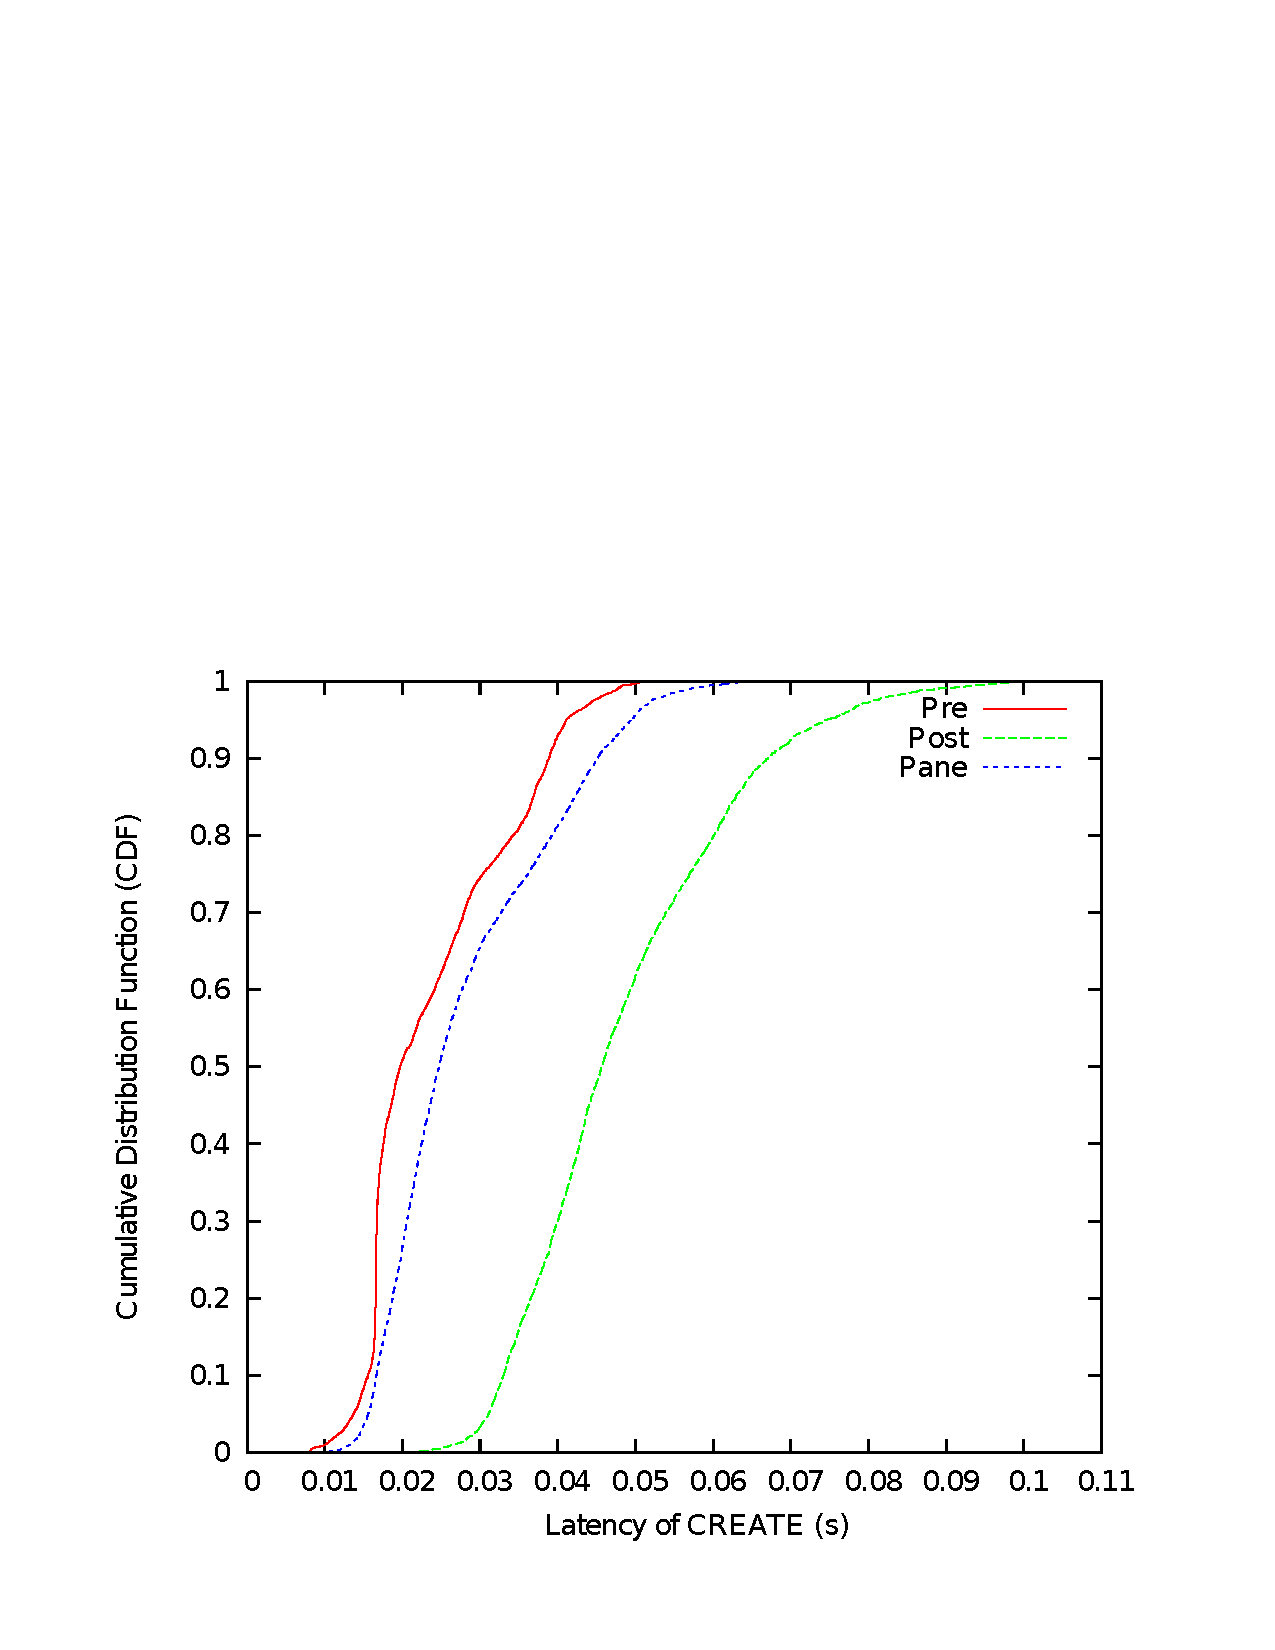
\includegraphics[width=0.5\textwidth, trim=0.5in 0.5in 0.5in 4.4in, 
%clip=true]{figs/create-latency-cdf-e}
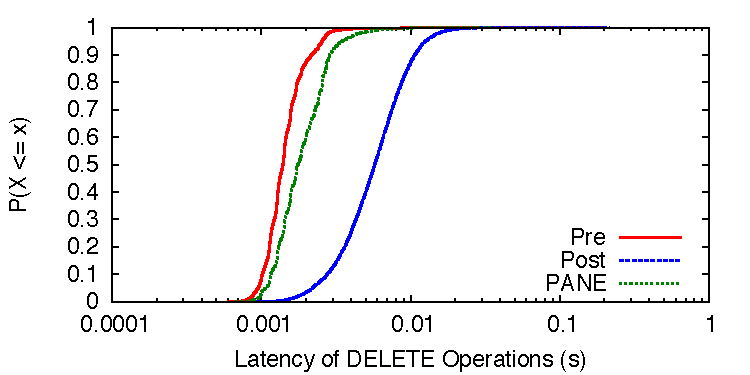
\includegraphics[width=\columnwidth]{figs/DELETE-zk-latencies-logscale}
\caption{Latency of ZooKeeper DELETE requests.}
\label{fig:ZooKeeperDELETE}
\end{figure}

Figure~\ref{fig:ZooKeeperDELETE} shows the latency of ZooKeeper DELETE requests 
during the experiment. In the ``Pre'' line, ZooKeeper alone is running in the 
network and no reservations were made using \sys. In the ``Post'' line, we used 
\verb/iperf/ to generate bi-directional TCP flows over each of the six links 
directly connected to a host.
%This traffic totaled 3.3 Gbps, which we found to 
%be the maximum Open vSwitch could sustain in our setup.
As shown in the 
figure, this competing traffic dramatically reduced ZooKeeper's performance -- 
average latency quadrupled from 1.55ms to 6.46ms (we obtained
similar results with a non-OpenFlow switch). Finally, the ``\sys'' line shows 
the return to high performance when ZooKeeper reserved bandwidth using \sys.

We found similar results for other ZooKeeper write operations such as creating 
keys, writing to unique keys, and writing to the same key. Read operations do 
not require a quorum's participation, and thus are less affected by competing background 
traffic.

\subsection{Hadoop}

\begin{figure}[t]
\centering
\subfigure[]{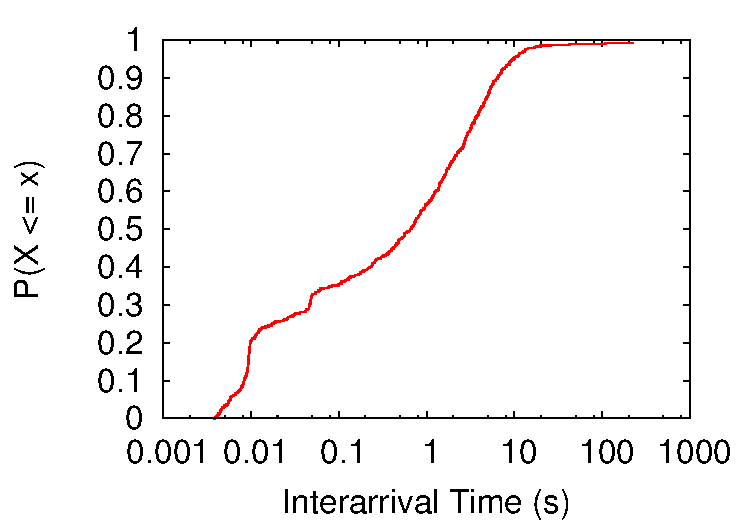
\includegraphics[width=0.23\textwidth]{figs/hadoop_reserv.pdf}}
\subfigure[]{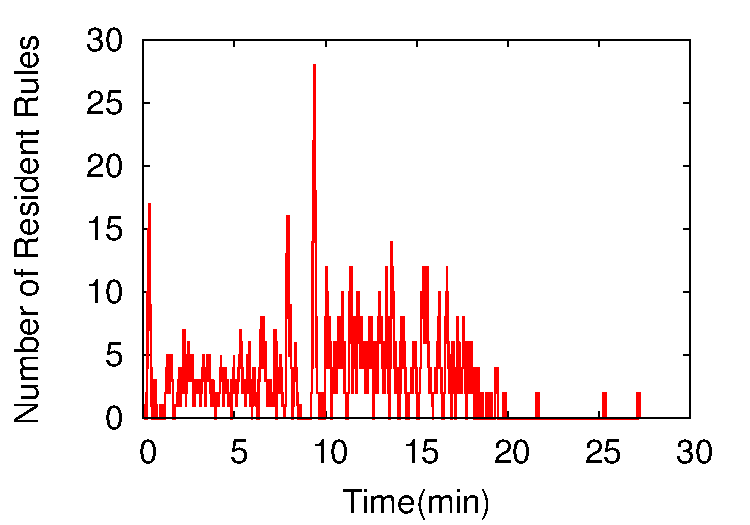
\includegraphics[width=0.23\textwidth]{figs/hadoop_resident_rules.pdf}}
\caption{Effect of Hadoop on \sys and network.}
\label{fig:HadoopResvs}
\end{figure}

In our final case study of \sys's application performance benefits, we augmented
a Hadoop 2.0.3 pre-release with support for our API. Hadoop is an open source
implementation of the MapReduce~\cite{Dean:2008} data-processing framework.
In Hadoop, large files are divided across multiple nodes in the network, and
computations consist of two phases: a map, and a reduce. During the
map phase, a function is evaluated in parallel on independent file pieces.
During the reduce, a second function proceeds in parallel on the collected outputs
of the map phrase; the data transfer from the mappers to the reducers is
known as the shuffle. During the shuffle, every reduce node initiates a
transfer with every map node, making it particularly network-intensive for
some jobs, such as sorts or joins.
Finally, the output of the reduce phase is written back to
the distributed filesystem (HDFS).

By using \sys, our version of Hadoop is able to reserve guaranteed bandwidth
for its operations. The first set of reservations occurs during the shuffle --
each reducer reserves bandwidth for transferring data from the mappers.
The second set of reservations reserves bandwidth when writing the
final output back to HDFS. These few reservations protect the majority of
network transfers that occur during the lifetime of a Hadoop job. Our
version of Hadoop also makes reservations when a map task needs to
read its input across the network; however, such transfers are typically
less common thanks to ``delay scheduling''~\cite{Zaharia:2010}.
Therefore, in a typical job, the total number of reservations is on the order of
$M \times R + R \times 2$ where $M$ and $R$ are, respectively, the
number of nodes with map and reduce tasks. The number of reservations
is not precisely described by this formula as we do not make reservations
for node-local transfers, and reducers may contact a mapper node more
than once during the shuffle phase.
As reducers can either be copying
output from mappers in the shuffle, or writing their output to HDFS,
the maximum number of reservations per reducer at any time is
set by the value of \emph{mapreduce.reduce.shuffle.parallelcopies}
in the configuration, which has a default value of five.

\vskip 0.5em

To measure the effect of using \sys to make reservations in Hadoop,
we developed a benchmark which executed three 40 GB sort jobs
in parallel on a network of 22 machines (20 slaves, plus two masters)
connected by a Pronto 3290 switched controlled by \sys.
Hadoop currently has the ability to prioritize or weight jobs using the
scheduler, but this control does not extend to the network.
In our benchmark,
the first two jobs were provided with 25\% of the cluster's memory
resources, and the third, acting as the ``high priority'' job, was provided
with 50\%. The benchmark was run in two configurations: in the first,
Hadoop made no requests using \sys; in the second, our modified
Hadoop requested guaranteed bandwidth for each large flow.
These reservations were proportional to the job's memory resources,
and lasted for eight seconds, based on Hadoop's 256 MB block size.
In our star topology with uniform 1 Gbps links, this translated to
500 Mbps reservations for each link. 

Averaged across three runs, the high priority job's completion
time decreased by 19\% when its bandwidth was guaranteed.
Because it completed more quickly, the lower priority jobs' runtime also
decreased, by an average of  9\%, since Hadoop's work-conserving scheduler re-allocates
freed memory resources to remaining jobs.

While Hadoop was running, we also measured its effect on \sys and
the switch's flow table. Figure~\ref{fig:HadoopResvs}(a) is a CDF of
the time between Hadoop's reservations. As currently implemented,
\sys modifies the switch flow table after each request. This CDF shows
that batching requests over a 10 ms window would decrease the
number of flow table updates by 20\%; a 100 ms window would decrease
the updates by 35\%. Figure~\ref{fig:HadoopResvs}(b) plots the amount
of flow table space used by Hadoop during a single job. On average,
Hadoop accounted for an additional 2.5 flow table entries; the maximum
number of simultaneous Hadoop rules was 28. 

\section{Implementation Practicality}
\label{sec:Microbenchmarks}

\begin{figure*}[t]
\centering
\subfigure[]{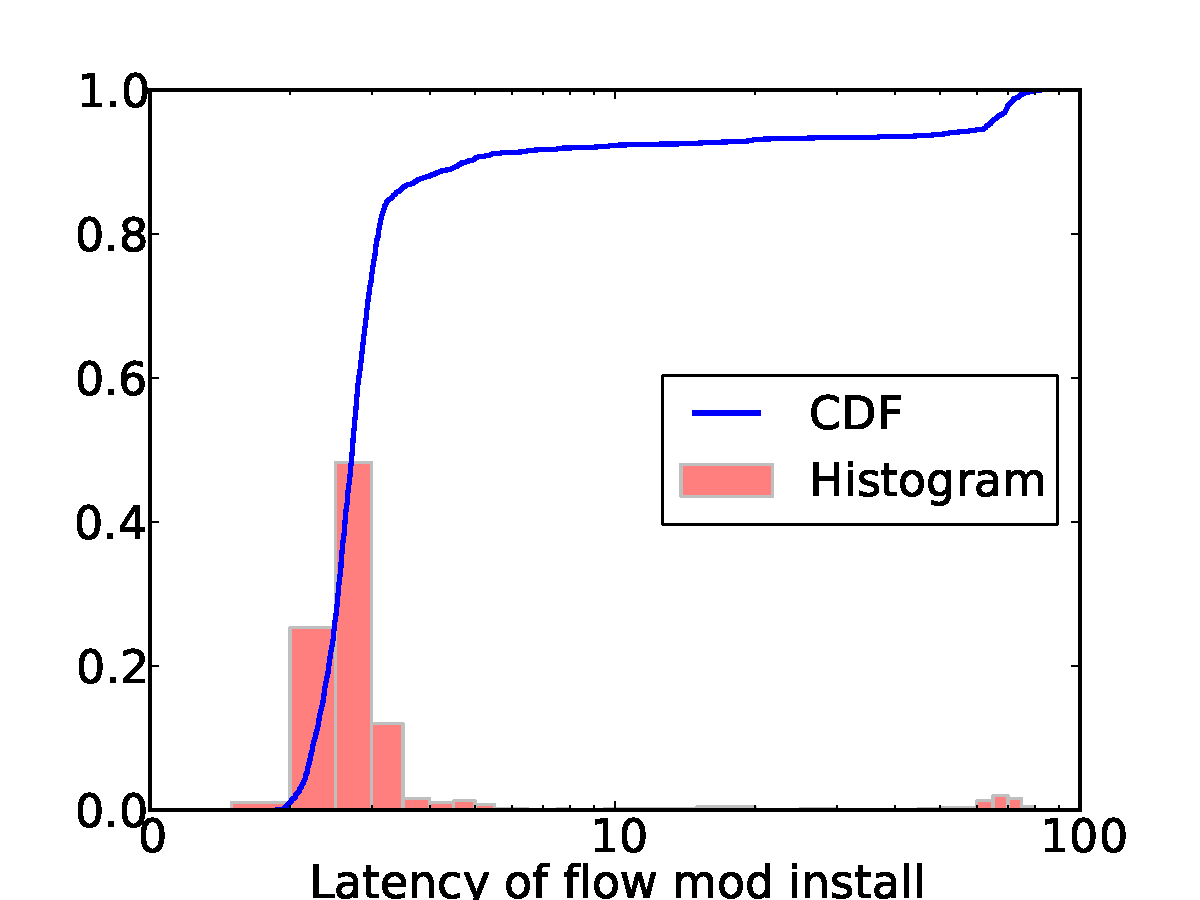
\includegraphics[width=0.25\textwidth]{figs/flow_mod-cdf.pdf}}
\subfigure[]{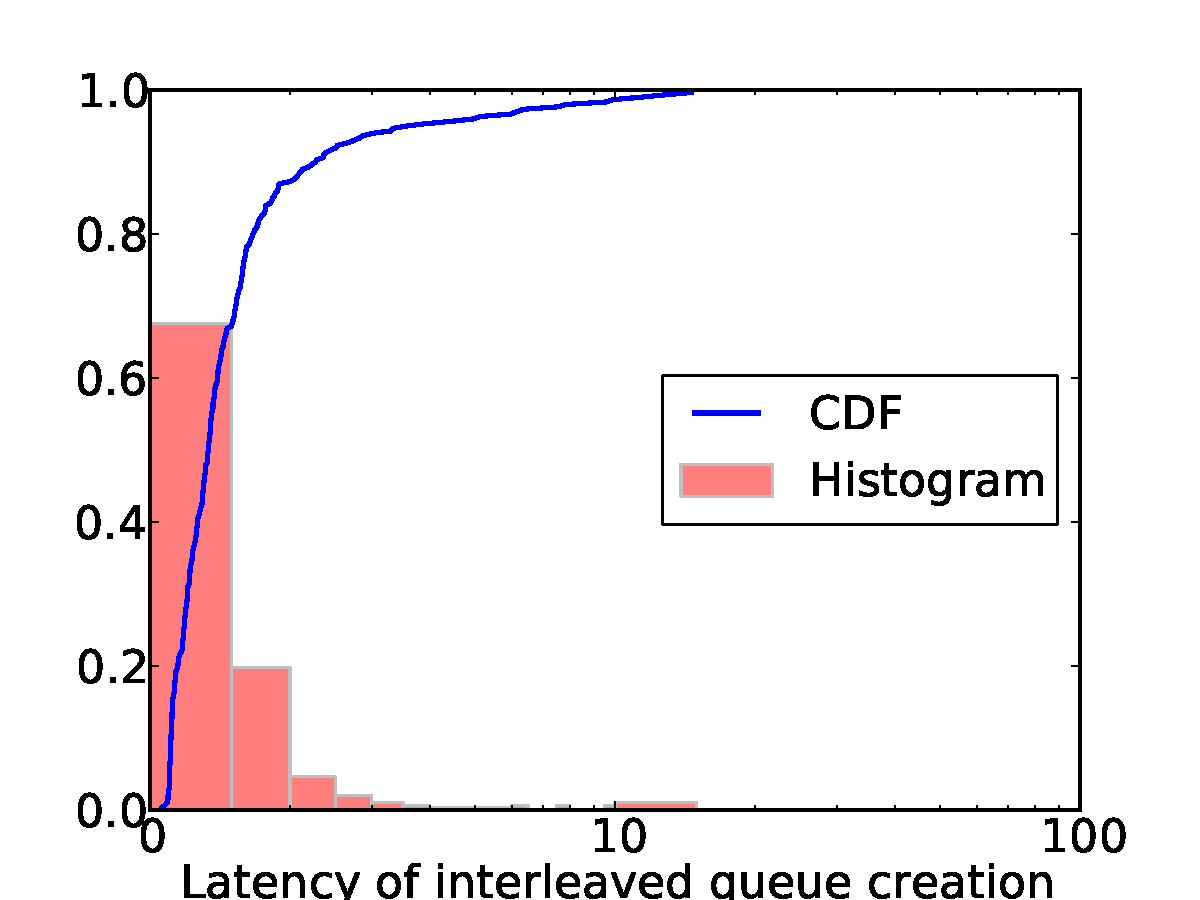
\includegraphics[width=0.25\textwidth]{figs/createQueue2-cdf.pdf}}
\subfigure[]{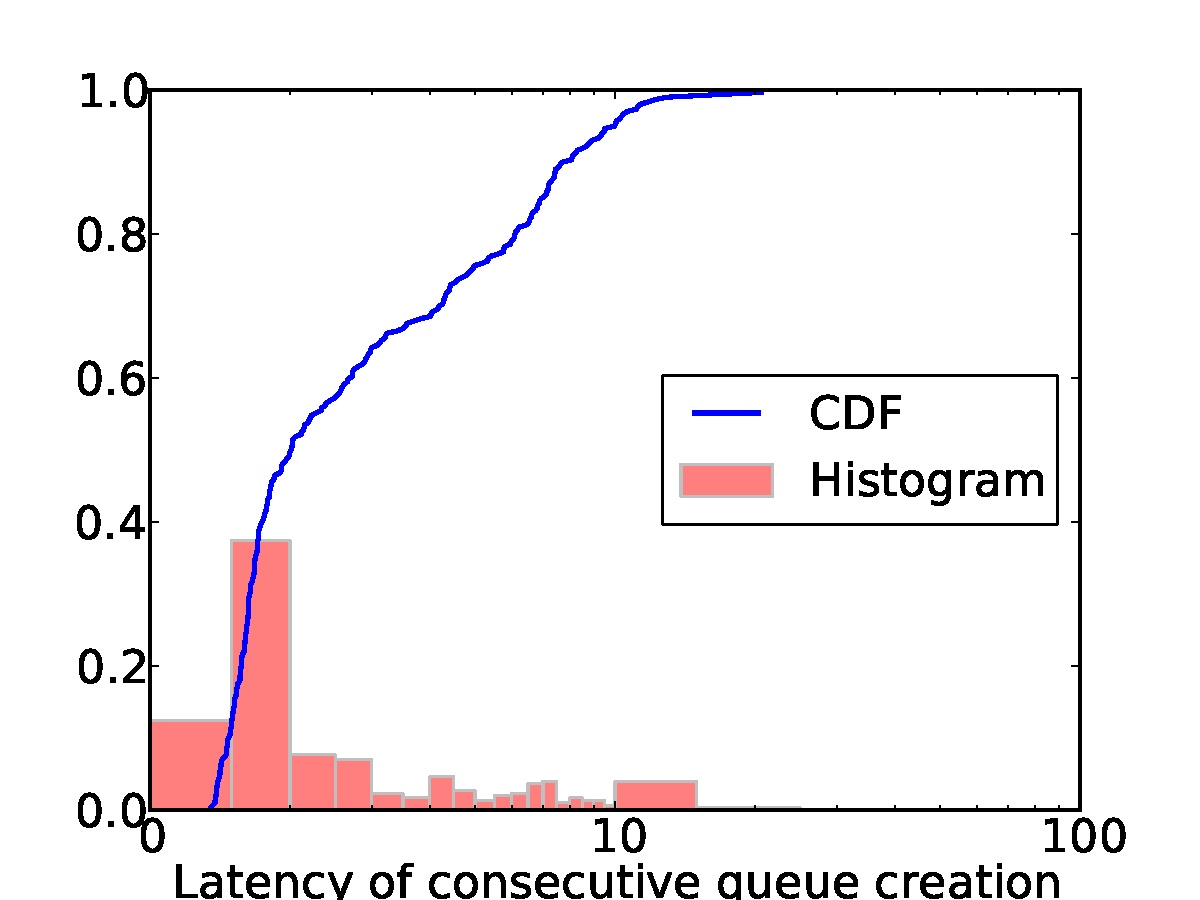
\includegraphics[width=0.25\textwidth]{figs/createQueue1-cdf.pdf}}
\caption{Latency of switch operations in milliseconds.}
\label{fig:SwitchOpLatency}
\end{figure*}

In addition to examining \sys's use in real applications, we also evaluated
the practicality of its implementation in current OpenFlow networks.
We found that our Pronto 3290 switches, running the Indigo 2012.09.07
firmware, were capable of supporting 1,919 OpenFlow rules, which took
an average of 7.12 ms to install per rule. To measure this, we developed a
benchmarking controller which installed wildcard match rules, issuing
a barrier request after each \verb/flow_mod/ message was sent. We based this
controller on Floodlight, and it is available for download from our Github page.

The latency distribution to fully install each \verb/flow_mod/ is show in
Figure~\ref{fig:SwitchOpLatency}(a). It has two clusters -- for the 92.4\% of
\verb/flow_mod/'s with latency less than 10.0 ms, the average latency
was 2.80 ms; the remaining 7.6\% had an average latency of 59.5 ms.
For \sys's principals, these much higher tail latencies imply that requests
cannot always be implemented within a few milliseconds, and for truly
guaranteed traffic handling, requests have to be made at least 100
milliseconds in advance.

We found that our Pronto switches could support seven hardware
queues with guaranteed minimum bandwidth on each port, and each
queue required an average of 1.73 ms to create or delete, as shown in
Figure~\ref{fig:SwitchOpLatency}(b). However, this average doubles to 3.56 ms
if queues are created consecutively on the same port (\ie, P1Q1, P1Q2,
P1Q3, ..., P2Q1, etc.), as shown in Figure~\ref{fig:SwitchOpLatency}(c).
This shows that an optimized \sys controller must consider the order in
which switch operations are made to provide the best experience.% for
%its principals.

Together, these results suggest that an
individual switch can support a minimum of about 200 reservations
per second. Higher throughput is possible by batching additional requests
between OpenFlow barriers.
While these switch features are sufficient to support the four applications
above, we found that Hadoop's performance benefited from per-flow
reservations only when flows transferred more than one megabyte. For
smaller flows, the overhead of establishing the reservations outweighed
the benefit.
In an example word count job, only 24\% of flows were greater
than 1 MB; however this percentage rises to 73\% for an example sort.
